\makeheading{2019-09-12}
\begin{remark}
    In integer programs, some examples of constraints that can be used are:
    \begin{itemize}
        \item $x_i\in\mathbb{Z}$
        \item $x\in\mathbb{Z}^n$
        \item $x_i\in\{0,1\}$
        \item $x_i$ is an integer
        \item $x_i\in\{0,1\}^n$
    \end{itemize}
\end{remark}

\begin{exbox}
    \begin{example}[Assignment Problem]
        SPIT has a campus near the North Pole. They have three buildings named
        A, B, C, which need to be renovated to be served as one of a
        Library, Laboratory, or Gym (sometimes called functions). Each
        building must be assigned one activity, and each activity must
        be assigned one building. Renovation costs in millions of
        dollars are given:

        \begin{center}
            \begin{tabular}{| *{4}{>{\centering\arraybackslash}p{3cm} |}}
                \hline
                  & Library & Laboratory & Gym \\ \hline
                A & 10      & 60         & 20  \\ \hline
                B & 60      & 70         & 50  \\ \hline
                C & 20      & 60         & 40  \\ \hline
            \end{tabular}\\
        \end{center}
        Find an assignment of activities to buildings so that the total
        renovation cost is minimized.

        \textbf{Solution.}
        Let us generalize to $n$ buildings and $n$ activities.
        \[
            x_{ij}:=
            \begin{cases}
                1 \text{, if $i$ is assigned to activity $j$} \\
                0 \text{, otherwise}
            \end{cases}
            \forall i,j\in\{1,\dots,n\}
        \]

        \[
            c_{ij}:=\text{renovation cost for assigning activity $j$ to building $i$}
        \]
        \begin{equation}
            \begin{aligned}
                 & \text{minimize}   & \quad & \sum\limits_{i = 1}^{n}\sum\limits_{j = 1}^{n}c_{ij}x_{ij}                                       \\
                 & \text{subject to} &       & \sum\limits_{i = 1}^{n}x_{ij}=1                            & \quad & \forall j\in\{1,\dots,n\}   \\
                 &                   &       & \sum\limits_{j = 1}^{n}x_{ij}=1                            & \quad & \forall i\in\{1,\dots,n\}   \\
                 &                   &       & x_{ij}=\{0,1\}                                             & \quad & \forall i,j\in\{1,\dots,n\} \\
                 &                   &       &
            \end{aligned}\tag{IP}
        \end{equation}
        \begin{itemize}
            \item First constraint $\implies$ every activity is assigned exactly one building
            \item Second constraint $\implies$ every building is assigned exactly one activity
            \item Third constraint $\implies $ $ x_{ij} $ is a \textbf{\emph{binary}} variable that takes
                  values only $ 1 $ or $ 0 $. If we wanted an IP formulation,
                  we would remove the constraint $ x_{ij}=\{0,1\} $
                  and add: $ x_{ij}\geqslant  0 $, $ x_{ij}\leqslant 1 $ and $ x_{ij} $ integer.
        \end{itemize}

    \end{example}
\end{exbox}

Suppose $c_{ij}\in\mathbb{R}$ and consider the inequality version
(if we don't assign \textbf{exactly} one item to another):
\begin{equation}
    \begin{aligned}
         & \text{minimize}   & \quad & \sum\limits_{i = 1}^{n}\sum\limits_{j = 1}^{n}c_{ij}x_{ij}                                       \\
         & \text{subject to} &       & \sum\limits_{i = 1}^{n}x_{ij}\leqslant 1                   & \quad & \forall j\in\{1,\dots,n\}   \\
         &                   &       & \sum\limits_{j = 1}^{n}x_{ij}\leqslant 1                   & \quad & \forall i\in\{1,\dots,n\}   \\
         &                   &       & x_{ij}=\{0,1\}                                             & \quad & \forall i,j\in\{1,\dots,n\} \\
         &                   &       &
    \end{aligned}\tag{IP}
\end{equation}
We can generalize this class optimization problem further.

\chapter{Introduction to Graphs}

\begin{defbox}
    \begin{definition}
        An \textbf{\emph{undirected graph}} is a pair $G=(V,E)$, where $V$ is a finite set
        of elements called \textbf{\emph{vertices}}, and $E$ is a set of pairs of distinct
        vertices called \textbf{\emph{edges}}. All edges in an undirected graph are bidirectional.
    \end{definition}
\end{defbox}

\begin{defbox}
    \begin{definition}
        Let $ G=(V,E) $ be a graph. Suppose $ uv\in E $. $ u,\,v $ are \textbf{\emph{adjacent}}
        vertices. $ u,\,v $ are the \textbf{\emph{endpoints}} of the edge $ uv $. The edge
        $ uv $ is \textbf{\emph{incident}} to vertices $ u $ and $ v $.
    \end{definition}
\end{defbox}
\begin{exbox}
    \begin{example}[Undirected Graph]
        Given $G:=$
        \[
            \begin{tikzpicture}
                \tikzstyle{LabelStyle}=[fill=white,sloped]
                \Vertex[x=0,y=4]{1}
                \Vertex[x=0,y=2]{2}
                \Vertex[x=2,y=2]{3}
                \Vertex[x=4,y=3]{4}
                \Vertex[x=3,y=1]{5}
                \Edge(1)(2)
                \Edge(3)(5)
                \Edge(2)(3)
                \Edge(3)(4)
                \tikzstyle{EdgeStyle}=[bend left]
                \Edge(2)(4)
                \Edge(1)(3)
            \end{tikzpicture}
        \]
        we have
        \[V=\{1,\dots,5\}\]
        \[E=\{12,13,23,24,35,34\}\]
    \end{example}
\end{exbox}

\begin{defbox}
    \begin{definition}
        Given a graph $G=(V,E)$, a \textbf{\emph{matching}} $M$ in $G$ is a subset of edges
        in $G$ such that no two edges in $M$ share a common vertex.
    \end{definition}
\end{defbox}
\begin{exbox}
    \begin{example}[Matching]
        In the above example:
        \begin{align*}
            \text{Matching}\qquad & \text{Not a Matching} \\
            M:=\{12\} \qquad      & M:=\{12,25\}          \\
            M:=\emptyset \qquad   & M:= \{67\}            \\
            M:=\{12,35\} \qquad
        \end{align*}
    \end{example}
\end{exbox}

\begin{defbox}
    \begin{definition}
        Given a graph $G=(V,E)$, if every vertex in $V$ of $G$ is
        an endpoint of an edge in $M$, we call
        the matching a \textbf{\emph{perfect matching}}.
    \end{definition}
\end{defbox}

The assignment problem is a special case of a
\emph{minimum cost perfect matching problem} or weighted graphs
(in this case every edge is given a weight/cost $c_{ij}$)

\[
    \begin{tikzpicture}
        \tikzstyle{LabelStyle}=[fill=white,sloped]
        \Vertex[x=0,y=3]{C}
        \Vertex[x=0,y=6]{B}
        \Vertex[x=0,y=9]{A}
        \Vertex[x=8,y=1]{Gym}
        \Vertex[x=8,y=6]{Lab}
        \Vertex[x=8,y=11]{Lib}
        \Edge[label=$10$](A)(Lib)
        \Edge[label=$60$](A)(Lab)
        \Edge[label=$20$](A)(Gym)
        \Edge[label=$60$](B)(Lib)
        \Edge[label=$70$](B)(Lab)
        \Edge[label=$50$](B)(Gym)
        \Edge[label=$20$](C)(Lib)
        \Edge[label=$60$](C)(Lab)
        \Edge[label=$40$](C)(Gym)
    \end{tikzpicture}
\]
\begin{remark}
    In a perfect matching graph, there are $n^2$ edges, and $2n$
    (an even number of) vertices.
\end{remark}